\begingroup
\setstretch{1}
\definecolor{archInk}{HTML}{3E5263}
\definecolor{archLine}{HTML}{B8C8D2}
\definecolor{archBlue}{HTML}{67BCEB}
\definecolor{archTeal}{HTML}{69D1AC}
\definecolor{archViolet}{HTML}{B69AE3}
\definecolor{archOrange}{HTML}{FAB875}
\definecolor{archRose}{HTML}{F48798}
\definecolor{archGold}{HTML}{F5D76E}
\definecolor{archFaceK}{HTML}{EBAC75}
\definecolor{archFaceI}{HTML}{86A8BB}
\definecolor{archFaceL}{HTML}{E3A09C}
\definecolor{archFaceJ}{HTML}{F1D48A}
\resizebox{1.10\linewidth}{!}{%
\begin{tikzpicture}[x=1mm,y=1mm,
  font=\sffamily\fontsize{12}{13}\selectfont,text=archInk,
  flow/.style={-{Latex[length=1.8mm,width=1.3mm]},draw=archInk!80,line width=.8pt},
  note/.style={font=\sffamily\fontsize{11}{12.5}\selectfont,align=center},
  heading/.style={align=center,font=\sffamily\bfseries\fontsize{13}{14.5}\selectfont},
  state/.style={draw=none,rounded corners=1mm,text width=23mm,minimum height=12mm,align=center},
  graphnode/.style={circle,draw=white,line width=.8pt,minimum size=6mm,
    inner sep=0,font=\sffamily\fontsize{10}{11}\selectfont}]
  \path[use as bounding box] (0,4) rectangle (238,-60);
  \node[heading] at (30,-56) {(A) B-Rep graph};
  \node[heading] at (116,-56) {(B) GNN and context};
  \node[heading] at (201,-56) {(C) Face labels};

  \node[note] at (16,-9) {Original B-Rep faces};
  \node[inner sep=0] at (16,-23)
    {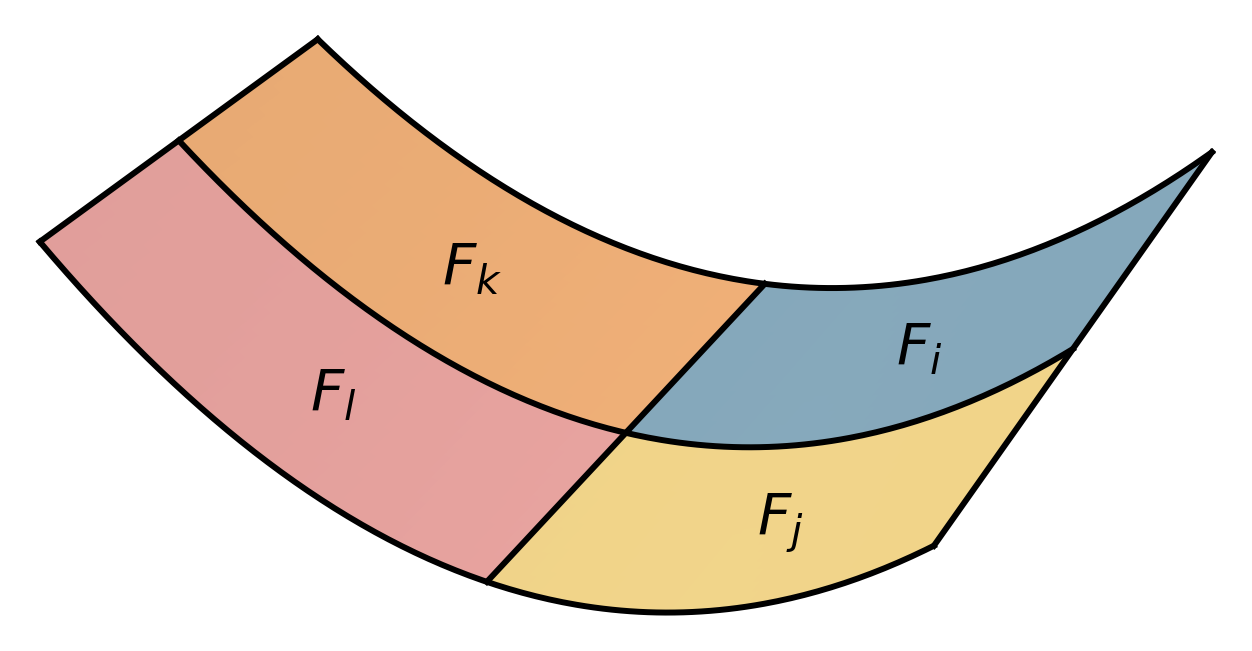
\includegraphics[width=32mm]{figures/fig5_bspline_curved_sheet.png}};
  \draw[flow] (33,-23) -- (39,-23);
  \node[note] at (50,-9) {Graph};
  \draw[archLine,line width=1pt] (43,-17) -- (57,-17) -- (57,-29) -- (43,-29) -- cycle;
  \foreach \x/\y/\name/\colour in {43/-17/k/archFaceK,57/-17/i/archFaceI,43/-29/l/archFaceL,57/-29/j/archFaceJ} {
    \node[graphnode,fill=\colour] at (\x,\y) {$v_{\name}$};
  }
  \node[note] at (50,-42) {Node: 48D\\Edge: 6D};
  \draw[flow] (62,-23) -- (72,-23);

  \foreach \offset/\colour in {9/archViolet,6/archTeal,3/archOrange,0/archBlue} {
    \path[fill=\colour!80,draw=\colour!70!black,line width=.5pt]
      (75+\offset,-14+\offset*.5) rectangle (88+\offset,-32+\offset*.5);
  }
  \node[note] at (81.5,-23) {64D};
  \node[note] at (85,-42) {NNConv $\times\,4$};
  \draw[archInk!80,line width=.8pt] (99,-23) -- (103,-23);
  \node[state,fill=archBlue!25] (local) at (120,-12) {Local\\64D};
  \node[state,fill=archTeal!27] (global) at (120,-34) {Global\\128D};
  \draw[flow] (103,-23) |- (local.west);
  \draw[flow] (103,-23) |- (global.west);
  \node[rounded corners=4mm,draw=none,fill=archViolet!35,minimum width=16mm,
    minimum height=10mm,inner sep=.5mm,font=\sffamily\fontsize{10.5}{12}\selectfont]
    (concat) at (149,-23) {Concat};
  \draw[flow] (local.east) -| (concat.north);
  \draw[flow] (global.east) -| (concat.south);
  \node[note] at (120,-47) {Mean $+$ max};
  \draw[flow] (concat.east) -- (165,-23);

  \foreach \ya in {-15,-20,-31} {
    \foreach \yb in {-15,-20,-31} {
      \draw[archLine!85,line width=.5pt] (170,\ya) -- (179,\yb);
    }
  }
  \foreach \ya in {-15,-20,-31} {
    \foreach \yb in {-17,-23,-29} {
      \draw[archLine!85,line width=.5pt] (179,\ya) -- (188,\yb);
    }
  }
  \foreach \y in {-15,-20,-31} {
    \node[circle,fill=archBlue,minimum size=3mm,inner sep=0] at (170,\y) {};
    \node[circle,fill=archViolet,minimum size=3mm,inner sep=0] at (179,\y) {};
  }
  \foreach \x in {170,179} {
    \node[fill=white,inner sep=.25mm,font=\fontsize{10}{11}\selectfont] at (\x,-25.5) {$\vdots$};
    \node[note] at (\x,-42) {192};
  }
  \foreach \y in {-17,-23,-29} {
    \node[circle,fill=archRose,minimum size=3mm,inner sep=0] at (188,\y) {};
  }
  \node[note] at (188,-42) {3};
  \node[note] at (179,-9) {MLP $+$ Linear};
  \draw[flow] (193,-23) -- (201,-23);
  \foreach \y/\colour/\name in {-14/{archLine!40}/Background,-23/archBlue/Rivet,-32/archOrange/{Cosmetic feature}} {
    \fill[\colour] (206,\y) circle (1.4mm);
    \node[note,anchor=west] at (210,\y) {\name};
  }
\end{tikzpicture}%
}
\endgroup
